\chapter{Examples in Matlab}

We now want to find approximate numerical solutions using Fourier spectral methods. In this section we focus primarily on the heat equation with periodic boundary conditions for $x\in[0,2\pi)$. Many of the techniques used here will also work for more complicated partial differential equations for which separation of variables cannot be used directly.
%%%%%%%
%Section
%%%%%%%
\section{1D Heat Equation}
The 1D heat equation
\begin{eqnarray}\label{eq:heat}
\frac{\partial u}{\partial t} = \alpha \frac{\partial^2 u}{\partial x^2}
\end{eqnarray}
is a well known second order PDE for which exact series solutions can be found using separation of variables.  It arises in several contexts such as in predicting the temperature in a thin uniform cross section rod. The equation and its derivation can be found in introductory books on partial differential equations and calculus, for example \cite{BoyDip10}, \cite{CouJoh98} and \cite{HugEtAl08},   The constant $\alpha$ is the thermal diffusivity and $u(x,t)$ is temperature. We have already described how to solve the heat equation using separation of variables. Let us first discretize $x$ such that $x_j$ where $j=0,1,2,...,n$. $x_j$ are uniformly spteaced in $[0,2\pi)$. Let's now take the FFT of both sides of the 1D heat equation to obtain
\begin{eqnarray}
\widehat{\frac{\partial u}{\partial t}} = \alpha \widehat{\frac{\partial^2 u}{\partial x^2}}.
\end{eqnarray}
We then rewrite the spatial derivative using eq.\ \eqref{eq:Spectral_Method_Deriv} \footnote{The $k$ subscript denotes the coefficient of the k$^{th}$ Fourier mode.}
\begin{eqnarray}
\frac{\partial \hat{u}_k}{\partial t} = \alpha (ik)^2 \hat{u}_k, 
\end{eqnarray}
so that the partial differential equation now becomes a collection of independent ODEs. While we can solve these ODEs in time exactly, we will use techniques that will also allow us to obtain approximate solutions to PDEs we cannot solve exactly. We will discuss two methods for solving these ODEs, forward Euler and backward Euler.

%subsection
\subsection{Forward Euler}
Using the forward Euler method in time, we obtain
\begin{eqnarray}
\frac{\hat{u}_k^{n+1}-\hat{u}_k^n}{h} = \alpha (ik)^2 \hat{u}_k^n \\
\hat{u}_k^{n+1} =\hat{u}_{k}^n+\alpha h(ik)^2\hat{u}_k^n  
\end{eqnarray}
All that is left is to take the IFFT of the computed solution after all timesteps are taken to transfer it back to real space. This is a linear PDE, so only one IFFT is needed at the end. We will later see that this is different for a nonlinear PDE. A Matlab implementation of this is in listing \ref{lst:HeatFE1dMatlab}.

\lstinputlisting[style=matlab_style,label=lst:HeatFE1dMatlab,caption={A Matlab program to solve the heat equation using forward Euler timestepping.}]{./ExamplesInMatlab/Programs/Heat_Eq_1D_Spectral_FE.m}
 
 %subsection
\subsection{Backward Euler}
To derive this method, we start by applying the FFT and then perform timestepping using backward Euler. We then rewrite the implicit form into a form that gives the next iterate,
\begin{eqnarray}
\frac{\partial \hat{u}_k}{\partial t} &=& \alpha (ik)^2 \hat{u}_k \\
\frac{\hat{u}_k^{n+1}-\hat{u}_k^n}{h} &=& \alpha (ik)^2 \hat{u}_k^{n+1} \\
\hat{u}_k^{n+1}(1-\alpha h(ik)^2) &=&\hat{u}_k^n\\
\hat{u}_k^{n+1} &=&\frac{\hat{u}_k^n}{(1-\alpha h(ik)^2)}.
\end{eqnarray}
Below is a graph of the numerical solution to the heat equation\footnote{Methods to obtain the exact solution can be found in, among other places,  Boyce and DiPrima~\cite{BoyDip10}. } where $n=64$ obtained using the Matlab program in listing \ref{lst:HeatBE1dMatlab}. 
\begin{figure}
 \begin{center}
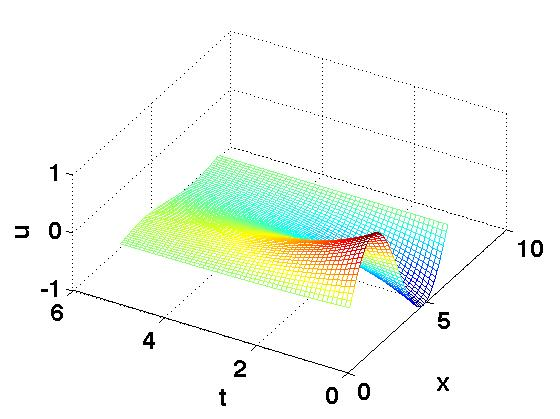
\includegraphics[scale=.35]{./ExamplesInMatlab/Heat_Equation_1D_BE_Color}
\caption{A numerical solution to the heat equation, eq.\ \eqref{eq:heat} computed using the backward Euler method.} \label{fig:HeatBE1dMatlab}
\end{center}
\end{figure}

\lstinputlisting[style=matlab_style,label=lst:HeatBE1dMatlab,caption={A Matlab program to solve the heat equation using backward Euler timestepping.}]{./ExamplesInMatlab/Programs/Heat_Eq_1D_Spectral_BE.m}

%subsection
\subsection{Exercises}
\begin{enumerate}
\item[1)] Write a program to solve the heat equation using the Crank-Nicolson method.
\item[2)] Solve the advection equation $u_t=u_x$ for $x\in[0,2\pi)$ with the initial data
\begin{enumerate}
\item[a)] $u(t=0,x)=\cos(x)$
\item[b)] $u(t=0,x)=\left\{{0\quad x<\pi}\atop{1\quad x\geq\pi}\right.$
\end{enumerate}
up to a time $T=1$. You can do this either by using separation of variables or by assuming that the solution is of the form $u(x,t)=f(x+t)$ and deducing what $f$ is in order to satisfy the initial conditions. In both cases please use the forward Euler, backward Euler and Crank-Nicolson timestepping schemes. After calculating the exact solution in each of these cases, examine how the maximum error at the final time depends on the timestep for each of these three methods.
\end{enumerate}


%%%%%%%
%Section
%%%%%%%
\section{Nonlinear Equations}
%subsection
\subsection{The 1D Allen-Cahn Equation}
So far we have dealt only with linear equations. Now it's time for a nonlinear PDE. The \emph{Allen-Cahn equation} models the separation of phases in a material. It was introduced by Sam Allen and J. W. Cahn~\cite{AllCah79}  and is 
\begin{eqnarray}
\frac{\partial u}{\partial t} = \epsilon\frac{\partial^2 u}{\partial x^2}+u-u^3, \label{eq:AllCah}
\end{eqnarray} 
where $\epsilon$ is a small but positive constant.  The way to numerically solve this is similar to the method used for the heat equation, but there are some notable differences. The biggest difference is that FFT($u^3$)$\neq$FFT($u$)$^3$, so the $u^3$ must be computed before taking the FFT. The FFT is a linear operation but cubing is non-linear operation, so the order matters
\begin{eqnarray}
\frac{\partial \hat{u}_k}{\partial t} = \epsilon\frac{\partial^2 \hat{u}_k}{\partial x^2}+\hat{u}_k-\widehat{u^3}_k. \label{Allen_Cahn_1D}
\end{eqnarray}
Next rewrite the first term on the right hand side, just like we did in the heat equation
\begin{eqnarray}
\frac{\partial \hat{u}_k}{\partial t} = \epsilon(ik)^2\hat{u}_k+\hat{u}_k-\widehat{u^3}_k.
\end{eqnarray}
In order to solve this numerically we are going to use a combination of implicit (backward Euler) and explicit (forward Euler) methods. We are going to skip forward Euler because it is unstable.

%subsubsection
\subsubsection{Implicit-Explicit Method} 
You might have already noticed that backward Euler is not going to work for the Allen-Cahn in its present state because of the nonlinear term. If you go to implement backward Euler you can see that you can't factor out all of the $\hat{u}_k^{n+1}$. Luckily there is a simple intuitive way around this that isn't detrimental to the accuracy of the solution. Write all the terms implicitly (backwards Euler) except for the nonlinear term which is expressed explicitly.  Applying this to Allen-Cahn we find that \footnote{Notice that when programming you are going to have to update the nonlinear term ($u^3$) each time you want to calculate the next timestep $n+1$. The reason this is worth mentioning is because for each timestep you are going to have to go from real space to Fourier space to real space, then repeat. For, the heat equation you can perform any number of timesteps in Fourier space and only convert back when you record your data.}
\begin{eqnarray}
\frac{\hat{u}_k^{n+1}-\hat{u}_k^n}{h} &=& \epsilon(ik)^2\hat{u}_k^{n+1}+\hat{u}_k^n-\widehat{(u^n)^3}_k \\
\hat{u}_k^{n+1}\left(-\epsilon(ik)^2+\frac{1}{h}\right)&=&\frac{1}{h}\hat{u}_k^n+\hat{u}_k^n-\widehat{(u^n)^3}_k \\
\hat{u}_k^{n+1}&=&\frac{\hat{u}_k^n(\frac{1}{h}+1)-\widehat{(u^n)^3}_k}{\left(-\epsilon(ik)^2+\frac{1}{h}\right)}. 
\end{eqnarray}
Now we have a form that we can work with. We can set the initial conditions to be $u(x,0)=\frac{1}{4} \sin(x)$ and plot the computed space-time evolution calculated by the Matlab code in listing \ref{lst:AllenCahnIE1dMatlab}. The computed result is in Fig.\ \ref{fig:AllenCahnIE1dMatlab}.

\lstinputlisting[style=matlab_style,label=lst:AllenCahnIE1dMatlab,caption={A Matlab program to solve the 1D Allen-Cahn equation using implicit explicit timestepping.}]{./ExamplesInMatlab/Programs/Allen_Cahn_1D_Spectral_IE.m}

\begin{figure}
\begin{center}
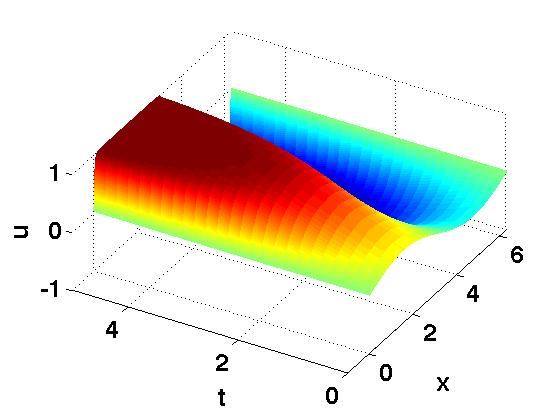
\includegraphics[scale=.2]{./ExamplesInMatlab/Allen_Cahn_BE_1D}
\caption{A numerical solution to the 1D Allen-Cahn equation, eq.\ \eqref{eq:AllCah}, with $\epsilon=0.001$ and $u(x,t=0)=0.25\sin(x)$ computed using an implicit explicit method.} \label{fig:AllenCahnIE1dMatlab}
\end{center}
\end{figure}

%subsection
\subsection{The 2D Allen-Cahn Equation}
Now we will look at the 2D form of the Allen-Cahn Equation, where $u(x,y,t)$ satisfies
\begin{eqnarray}
\frac{\partial u}{\partial t} = \epsilon\left(\frac{\partial^2 u}{\partial x^2}+\frac{\partial^2 u}{\partial y^2}\right)+u-u^3. \label{eq:AllCah2D}
\end{eqnarray}
The convert it into Fourier space by taking the FFT of both sides
\begin{eqnarray}
\frac{\partial \hat{u}_k}{\partial t} &=& \epsilon\left(\frac{\partial^2 \hat{u}_k}{\partial x^2}+\frac{\partial^2 \hat{u}_k}{\partial y^2}\right)+\hat{u}_k-\widehat{u^3}_k\\
\frac{\partial \hat{u}_k}{\partial t} &=& \epsilon\left((ik_x)^2\hat{u}_k+(ik_y)^2\hat{u}_k\right)+\hat{u}_k-\widehat{(u^3)}_k \label{eq:Allen_Cahn_2D}
\end{eqnarray}
where $k_x$ and $k_y$ is to remind us that we take the FFT in respected directions. We will also define
\begin{eqnarray}
f(u) \equiv u-u^3 \label{eq:nonlinear}
\end{eqnarray}
The way to deal with the first two terms on the right hand side is to take the FFT in the x-direction and then take it in the y-direction. The order in which the FFT is done, $x$ first or $y$ first is not important. Some software libraries offer a two dimensional FFT. It usually depends on the equation being solved whether it is more efficient to use a multidimensional FFT or many one dimensional FFTs. Typically, it is easier to write a program which uses a multidimensional FFT, but in some situations this is not very efficient since one can immediately reuse data that has just been Fourier transformed.
%subsubsection
\subsubsection{Implicit-Explicit Method}
In this method, the nonlinear term in eq.\ \eqref{eq:nonlinear} is calculated explicitly, while the rest of the terms will be written implicitly such that
\begin{align}
&{} \frac{\hat{u}_k^{n+1}-\hat{u}_k^n}{h} = \epsilon\left((ik_x)^2\hat{u}_k^{n+1}+(ik_y)^2\hat{u}_k^{n+1}\right)+\widehat{f(u^n)}_k 
\\&{} \hat{u}_k^{n+1}\left(-\epsilon(ik_x)^2-\epsilon(ik_y)^2+\frac{1}{h}\right)=\frac{\hat{u}_k^n}{h}+\widehat{f(u^n)}_k
\\&{} \hat{u}_k^{n+1} = \frac{\frac{\hat{u}_k^n}{h}+\widehat{f(u^n)}_k}{ \left(-\epsilon(ik_x)^2-\epsilon(ik_y)^2+\frac{1}{h}\right)}
\end{align}
we can then substitute in for $f(u)$
\begin{align}
\hat{u}_k^{n+1} = \frac{\hat{u}_k^n\left(\frac{1}{h}+1\right)-\widehat{(u^n)^3}_k}{ \left(-\epsilon(ik_x)^2-\epsilon(ik_y)^2+\frac{1}{h}\right)}. \label{eq:Allen_Cahn_IE_2D}
\end{align}
\begin{figure}
\begin{center}
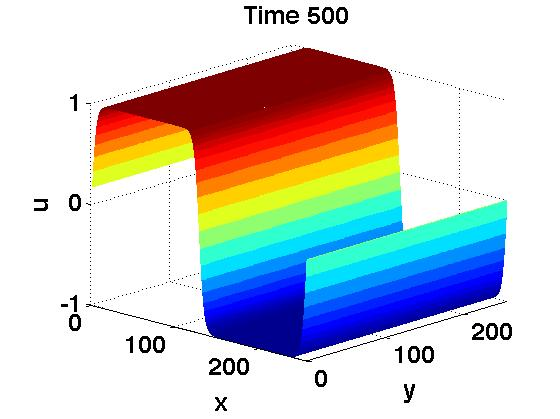
\includegraphics[scale=.2]{./ExamplesInMatlab/Allen_Cahn_2D_IE}
\caption{A numerical solution to the 2D Allen-Cahn equation, eq.\ \eqref{eq:AllCah2D} at time $t=500$ with $\epsilon=0.1$ and $u(x,y,t=0)=\sin(2\pi x)+0.001\cos(16\pi x)$ computed using an implicit explicit method.} \label{fig:AllenCahnIE2dMatlab}
\end{center}
\end{figure}
The Matlab code used to generate Fig.\ \ref{fig:AllenCahnIE2dMatlab} is in listing \ref{lst:AllenCahnIE2dMatlab}.

\lstinputlisting[style=matlab_style,label=lst:AllenCahnIE2dMatlab,caption={A Matlab program to solve the 2D Allen-Cahn equation using implicit explicit timestepping.}]{./ExamplesInMatlab/Programs/Allen_Cahn_2D_Spectral_IE.m}

%subsection
\subsection{Exercises}

Many of these exercises are taken from Uecker~\cite{Uec09}. Another introductory source of information on these equations is Trefethen and Embree~\cite{TreEmb01}.

\begin{enumerate}
\item[1)] Burgers equation is given by:
$$\frac{\partial u}{\partial t}=\nu \frac{\partial^2 u}{\partial x^2} - u\frac{\partial u}{\partial x}$$
where $\nu\in\mathbb{R}^+$ and $u$ has periodic boundary conditions. Solve this equation using an implicit-explicit method. If you take $\nu$ to be small, ensure that a sufficient number of grid points are used to get the correct numerical solution. A simple way to check this is to keep increasing the number of grid points and checking that there is no change in the solution. Another way to check this is to calculate the Fourier coefficients and check that the highest ones decay to machine precision. 
\item[2)] The Kuramoto-Sivashinsky equation is given by:
$$\frac{\partial u}{\partial t}=-\frac{\partial^2 u}{\partial x^2}-\frac{\partial^4 u}{\partial x^4}-u\frac{\partial u}{\partial x}$$
where $u$ has periodic boundary conditions.
\begin{itemize}
\item[a)] What does this equation model and what type of behavior do you expect its solutions to have?
\item[b)] Find numerical solutions to this equation using an implicit-explicit method.
\end{itemize}
\item[3)] The 1D Gray-Scott equations are given by:
$$\frac{\partial u}{\partial t}=d_1\frac{\partial^2 u}{\partial x^2}-uv^2+f(1-u),$$
$$\frac{\partial v}{\partial t}=d_2\frac{\partial^2 v}{\partial x^2} + uv^2 - (f+k)v$$
where $d_1$, $d_2$, $f$ and $k$ are constants. 
\begin{itemize}
\item[a)] What does this equation model and what type of behavior do you expect its solutions to have?
\item[b)] Find numerical solutions to this equation using an implicit-explicit method. Try several different values of $d_1$, $d_2$, $f$ and $k$ and compare the resulting patterns to what you can find in the literature.
\end{itemize}
\item[4)] The 2D Swift-Hohenberg equation is given by:
$$\frac{\partial u}{\partial t}=-\Delta^2u+2\Delta u+ (\alpha-1)u-u^3,$$
\begin{itemize}
\item[a)] What does this equation model and what type of behavior do you expect its solutions to have?
\item[b)] Find numerical solutions to this equation using an implicit-explicit method for several values of $\alpha$.
\end{itemize}
\item[5)] The 2D Gray-Scott equations are given by:
$$\frac{\partial u}{\partial t}=d_1\Delta u -uv^2+f(1-u)$$
$$\frac{\partial v}{\partial t}=d_2\Delta v  + uv^2 - (f+k)v$$
where $d_1$, $d_2$, $f$ and $k$ are constants. 
\begin{itemize}
\item[a)] What does this equation model and what type of behavior do you expect its solutions to have?
\item[b)] Find numerical solutions to this equation using an implicit-explicit method.
\end{itemize}
\item[6)] The 2D Complex Ginzburg-Landau equation is given by:
$$\frac{\partial A}{\partial t}=A+(1+i\alpha)\Delta A- (1+i\beta)|A|^2A.$$
An introductory tutorial to this equation can be found at \url{http://codeinthehole.com/static/tutorial/index.html}
\begin{itemize}
\item[a)] What does this equation model and what type of behavior do you expect its solutions to have?
\item[b)] Find numerical solutions to this equation using an implicit-explicit method for several values of $\alpha$ and $\beta$.
\end{itemize}
\end{enumerate}
